% Figure from MATH 591 notes, section 71. Compile with the notes preamble.
\begin{tikzpicture}[>=stealth, scale=0.95]
\draw[->, gray!70] (-0.6,-3.0) -- (-0.6,3.4) node[above, font=\scriptsize, text=black] {$\mathfrak{u}(1) = i\mathbb{R}$};
\draw[blue!70!black, line width=2pt] (-0.6,0) -- (-0.6,2.639);
\draw[red!70!black, line width=2pt] (-0.6,-1.319) -- (-0.6,0);
\fill (-0.6,0.000) circle (1.4pt) node[left, font=\scriptsize] {$0$};
\fill (-0.6,0.660) circle (1.4pt) node[left, font=\scriptsize] {$\tfrac{\pi}{2}i$};
\fill (-0.6,1.319) circle (1.4pt) node[left, font=\scriptsize] {$\pi i$};
\fill (-0.6,1.979) circle (1.4pt) node[left, font=\scriptsize] {$\tfrac{3\pi}{2}i$};
\fill (-0.6,2.639) circle (1.4pt) node[left, font=\scriptsize] {$2\pi i$};
\fill (-0.6,-0.660) circle (1.4pt) node[left, font=\scriptsize] {$-\tfrac{\pi}{2}i$};
\draw[->, thick] (0.4,0.9) -- node[above, font=\scriptsize] {$\exp$} (1.7,0.9);
\draw[gray!50] (1.9,0.6) -- (5.9,0.6); \draw[gray!50] (3.9,-1.4) -- (3.9,2.6);
\draw[blue!70!black, line width=2pt] (3.9,0.6) ++(0:1.5) arc (0:360:1.5);
\draw[red!70!black, line width=1pt] (3.9,0.6) ++(0:1.38) arc (0:-180:1.38);
\fill (5.400,0.600) circle (1.4pt) node[right, font=\scriptsize] {$1 = e^{0} = e^{2\pi i}$};
\fill (3.900,2.100) circle (1.4pt) node[above right, font=\scriptsize] {$i$};
\fill (2.400,0.600) circle (1.4pt) node[left, font=\scriptsize] {$-1$};
\fill (3.900,-0.900) circle (1.4pt) node[below right, font=\scriptsize] {$-i$};
\node[font=\scriptsize] at (5.45,2.25) {$\mathrm{U}(1)$};
\node[font=\scriptsize, align=left, anchor=north west] at (-0.4,-1.9) {blue: $[0, 2\pi i]$, once around;\\ red: $[-\pi i, 0]$, the lower half again};
\end{tikzpicture}
